% COSC 4P03 Project
% sudoku generator
% Taras Mychaskiw

\section{Results}

A sample of $100,000$ ($10$ sets of $10,000$) sudoku puzzles were generated using each of the generation strategies discussed above.
During each of these, all three sudoku solvers were run concurrently to check formity of a puzzle. Once one solver got the answer,
it would return the answer and the other two would stop calculating. The "winner" (the solver that took the least amount of time) of each
of these was stored for an additional comparison of the solvers. All the results below (to do with this set) are are an average over
the $10$ runs, each of which calculated the average over generating $10,000$ sudoku puzzles.

\subsection{Comparison of Solving Strategies}

    \subsubsection{Solving Hard Puzzles}
    To compare the solving strategies, each of them were used to solve all of Peter Norvig's Top 95 sudoku puzzles\cite{norvig}.
    These puzzles are considered some of the hardest ever found. Each of the solvers solved each puzzle, and checked the formity
    of each puzzle as well.
    \begin{table}[H]
    \begin{center}\begin{tabular}{l|r|r}
        \hline
        Solver          &   Total Time to Solve     &   Total Time to Check Formity \\  \hline
        Backtracking    &   $593475$ms              &   $1407571$ms                 \\
        Constraint      &   $243$ms                 &   $351$ms                     \\
        Exact Cover     &   $166$ms                 &   $99$ms                      \\
        \hline
    \end{tabular}\end{center}
    \label{tab:top95}
    \caption{Results of each of the solvers solving and checking the formity of Peter Norvig's Top 95 sudoku puzzles.}
    \end{table}
    Seems that exact cover and dancing links is far ahead of the competition. Constraint propagation didn't do too badly. Backtracking
    is just not as good as the other two. Something to note about the formity time for exact cover - it's less than the time to took
    to solve the same puzzles. Seems counter intuitive, but it has to do with how the solving was actually implemented. Solving a puzzle
    would return the solved version of the puzzle, while formity checking only returned an integer. In exact cover, post processing is
    required to convert the matrix back into a sudoku board, but this is not required in checking the formity. All that matters for formity
    is that a new solution was found (if it was), the actual solution is not overly important.
    %\end{Solving Hard Puzzles}
    
    \subsubsection{Use in Generation}
    Something surprising happened during generation - backtracking still won. It seems that, from the data above, backtracking would
    win very few times if at all. It was excepted that exact cover would be about $60\%$ of the wins, and constraint propagation would
    be about $35\%$. However, this was not the case. Figure~\ref{fig:solvergen} should the results of the winners during the generation.
    \begin{figure}[H]
        \centering
        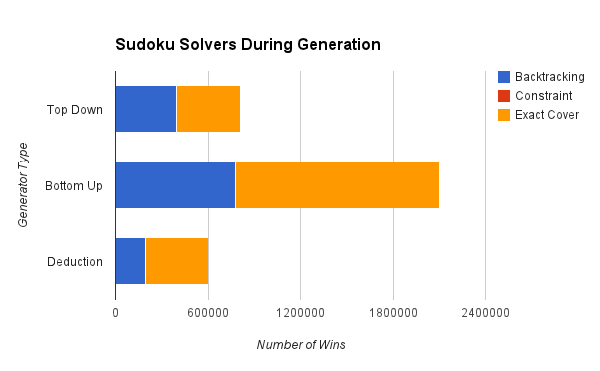
\includegraphics[scale=0.70]{solvers.png}
        \caption{Results of how many times each solver won during each of the generation of sudoku puzzles.}
        \label{fig:solvergen}
    \end{figure}
    As expected, exact cover does win about $60\%$ of the time. However backtracking and constraint propagation are backwards (note this
    was \textit{not} an implementation issue!). In fact, constraint propagation won so few times that it doesn't even appear in the graph.
    So why did backtracking do much better than expected? For top down generation, it actually makes sense. Backtracking requires absolutely
    no pre- or post-processing of the data. It just loops through the board, skipping clues already given in the puzzle. During top down generation,
    most of the puzzle is already given, so backtracking has very few calculations to actually do. Meanwhile, constraint propagation and exact
    cover are still pre-processing the board. Backtracking would win while the board is fairly full still, then later exact cover would outperform.
    And that's exactly the results we for the top down generation.\\
    What about bottom up and deduction generation? Each of those start with an empty board that the solvers would run on. Backtracking is still
    a major contender. The difference between the results in the previous section and now is that the formity checks are on boards that are
    not well formed, they usually have more than one solution. Each of the solving strategies is a depth first search, so if there are many
    solutions, they would find two similar ones quickly and return that there are multiple solutions. The difference between backtracking
    and the others is again the lack of additional processing. On a near empty sudoku, basically any values you throw into a cell will lead
    to a solution with very little backtracking actually required. So, the same reasoning applies. While exact cover is still pre-processing,
    backtracking has gotten a head start, and may end up finding two very similar solutions very quickly and winning.\\
    Constraint propagation didn't do anywhere near as well as expected. This is likely due to the unexpected backtracking results. Backtracking
    does exceptionally well in near full and near empty boards while checking for formity. In all other cases, exact cover would simply outperform
    constraint propagation. Given these facts, it makes sense that constraint propagation simply fails to show any results. If one were to redo
    the experiment without using exact cover, my personal estimate is that constraint propagation would take exact cover's position and win
    most of the time.
    %\end{Use in Generation}

%\end{Comparison of Solving Strategies}

\subsection{Comparison of Generation Strategies}
\begin{figure}[H]
    \centering
    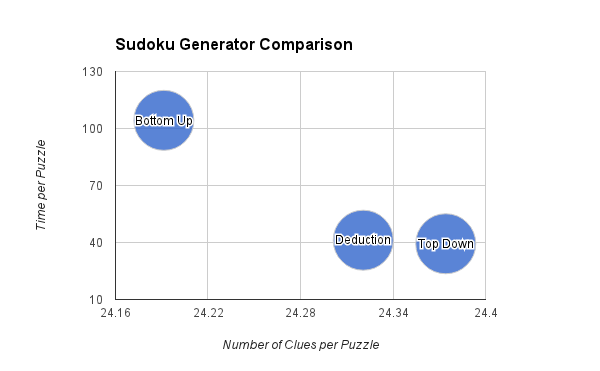
\includegraphics[scale=0.70]{generators.png}
    \caption{Results of generators.}
    \label{fig:generators}
\end{figure}
%\end{Comparison of Generation Strategies}

%\end{Results}
